
\subsection{Intellectual Property core}

An IP core, or intellectual property (IP) core, is a
pre-designed and tested digital logic circuit that can be easily integrated
into a larger system on a chip (SoC) or field-programmable gate array (FPGA).
IP cores are designed to perform specific functions, such as data processing,
communication or  system control, and can be used to quickly add these
functions to a design without having to design them from scratch.

\subsubsection{Make vs buy decision}
The decision of whether to make or buy an IP core for a hardware
design can depend on a number of factors. This factors range from cost,
time-to-market, quality, customization and retaining the intellectual
property of the product.

    Developing an IP core in-house can seem cheaper as opposed to
buying it from a third-party company in the first place. However, in the long
run, resource and time costs for designing and testing the core may become
greater than buying. Buying can also lead to significantly lower
time-to-market.

    Buying an IP core from an established developer can give the
guarantee of a higher quality product with less defects, given that the
company specializes in core design and continuously works on perfecting their
products.

    In cases of very specific uses, where there aren't any
commercially available cores, it may be needed to develop a custom design
in-house. Making this choice gives the benefit of maintaining the IP rights
to the core and opens the possibility of later retailing it.

    Ultimately the decision of making vs buying will depend on the
specific needs of the project and its final goal.

\subsubsection{IP core Business Model}
The IP core business model is a business strategy that focuses
on creating, licensing and selling Intellectual Property assets. Dealing in
the IP business has the advantage of being able to generate revenue from
selling use licenses of IP assets, without ever having to actually
manufacture the product. Companies in the IP market can remain focused on
researching and developing new products without worrying with production and
distribution of said products.

\subsection{The Internet of Things}
The Internet of Things (IoT) is generally defined as the
extensibility of network, computation and sensor capabilities to everyday
objects, typically not capable of such features. This allows for an
inter-connectivity between this devices and the rest of the internet, making
them capable of generating, exchanging and consuming data between themselves
and the cloud.

\subsubsection{Network Interface IP cores in IoT}
Even though IoT devices exist across all types of applications
and use cases, all of them share the need to be connected. Network Interfaces
provide this necessary connectivity through hardware and software designed to
handle the networking protocols.

    The use of IP Network Interface cores greatly simplifies the
design and development of IoT devices, as they provide a tested solution that
can be easily installed in the system through standard protocols. This IP
cores also ensure that the device is interoperable with other systems, using
standard networking protocols.

    Given the variety of applications for IoT devices, it would be
unfeasible for developers to design a new interface for each device. Luckily
there already exist a vast array of Network Interface IP cores that are
specialized and optimized in different aspects that range from speed of
connection to power-saving utilities or even all sorts of network protocols.

\subsection{Network Protocol Layers}
As defined in the OSI (Open System Interconnection) reference
model, the Network Protocol is comprised of 7 layers, where each layer is
responsible for a specific aspect of communication.

\begin{figure}[H]
    \centering
    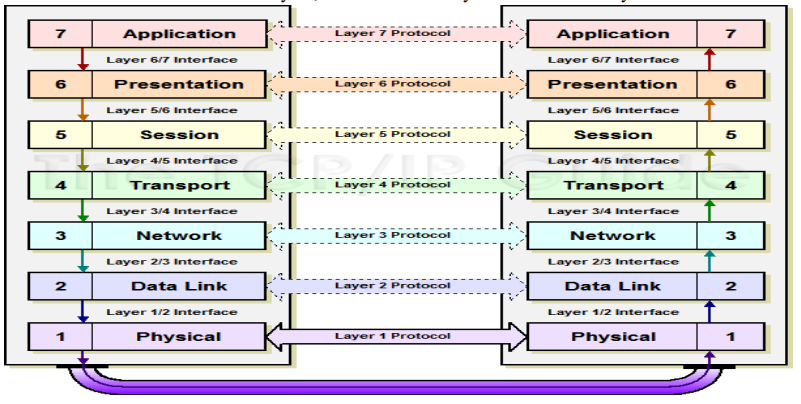
\includegraphics[scale=0.38]{osi model.png}
    \caption{Network Protocol Layers}
    \label{fig:osi_model}
\end{figure}

As seen in figure~\ref{fig:osi_model}, layers 1 (Physical), 2 (Data Link) and 3
(Network) are at the lower levels of the network protocol. As such, Network
Interface IP cores mostly belong within these layers.

\subsubsection{Physical Layer}
Normally implemented with a dedicated chip or a specialized IP
core, this layer is responsible for defining the physical and electrical
specifications between the device and the transmission medium. The modulation
(or conversion) of information is also done at this level, depending on the
physical communication channel.

\subsubsection{Data Link Layer}
The second lowest layer of the network protocol, the data link
layer is responsible for providing reliable transmission of data between
adjacent devices, using a set of protocols that are built on top of the raw
and unreliable transmission service provided by the physical layer. To ensure
reliable transmission, the data link layer performs error detection and
correction, typically using a Cyclic Redundancy Check (CRC). The Ethernet
protocol runs at this layer.

\subsubsection{Network Layer}
While the previous 2 layers deal with transmitting/receiving data
and checking for its integrity, the network layer is responsible for
addressing the packets before transmission. Every device has a specific
address with which it is known on a network and by effectively addressing
each packet, the information can easily reach its intended destination within
a network. This addressing is done through the Internet Protocol (IP
protocol), that runs in this layer.

    Specific UDP related hardware runs on this layer, on top of the
IP protocol, and is responsible for dealing with low-level details of
assembling and disassembling UDP packets.

\subsubsection{Transport Layer}
The transport layer is responsible for a number of things. It
establishes, terminates and maintains connections, implements congestion,
flow and error control mechanisms and most of all it is through this layer
that the application programmers interact with the lower layers, so it must
run the necessary software drivers for the underlying hardware.


\subsection{IOBundle Ethernet core}
citation tests~\cite{rec2020,bib:riscv_list}~